%%%%%%%%%%%%%%%%%%%%%%%%%%%%%%%%%%%%%%%%%
% Chair of Cyber-Physical-Systems
% Univ.-Prof. Dr. Elmar Rueckert
% Montanuniversität Leoben, Austria
% Latest Update: Feb. 2022
%
% Disclaimer: The materials and source code are for personal use only. The material is intended for educational purposes only. Reproduction of the material for any purposes other than what is intended is prohibited. The content is to be used for educational and non-commercial purposes only and is not to be changed, altered, or used for any commercial endeavor without the express written permission of Professor Rueckert. 
% 
% Original Version by Frits Wenneker, 28/2/17,  License: CC BY-NC-SA 3.0 (http://creativecommons.org/licenses/by-nc-sa/3.0/)
%%%%%%%%%%%%%%%%%%%%%%%%%%%%%%%%%%%%%%%%%

%----------------------------------------------------------------------------------------
%	PACKAGES AND OTHER DOCUMENT CONFIGURATIONS
%----------------------------------------------------------------------------------------

\documentclass[10pt, a4paper, twocolumn]{article} % 10pt font size (11 and 12 also possible), A4 paper (letterpaper for US letter) and two column layout (remove for one column)

%%%%%%%%%%%%%%%%%%%%%%%%%%%%%%%%%%%%%%%%%
% Chair of Cyber-Physical-Systems
% Univ.-Prof. Dr. Elmar Rueckert
% Montanuniversität Leoben, Austria
% Latest Update: Feb. 2022
%
% Disclaimer: The materials and source code are for personal use only. The material is intended for educational purposes only. Reproduction of the material for any purposes other than what is intended is prohibited. The content is to be used for educational and non-commercial purposes only and is not to be changed, altered, or used for any commercial endeavor without the express written permission of Professor Rueckert. 
% 
% Original Version by Frits Wenneker, 28/2/17,  License: CC BY-NC-SA 3.0 (http://creativecommons.org/licenses/by-nc-sa/3.0/)
%%%%%%%%%%%%%%%%%%%%%%%%%%%%%%%%%%%%%%%%%

%----------------------------------------------------------------------------------------
%	PACKAGES AND OTHER DOCUMENT CONFIGURATIONS
%----------------------------------------------------------------------------------------

\usepackage[english]{babel} % English language hyphenation

\usepackage{microtype} % Better typography

\usepackage{amsmath,amsfonts,amsthm} % Math packages for equations

\usepackage[svgnames]{xcolor} % Enabling colors by their 'svgnames'

\usepackage[hang, small, labelfont=bf, up, textfont=it]{caption} % Custom captions under/above tables and figures

\usepackage{booktabs} % Horizontal rules in tables

\usepackage{lastpage} % Used to determine the number of pages in the document (for "Page X of Total")

\usepackage{graphicx} % Required for adding images

\usepackage{enumitem} % Required for customising lists
\setlist{noitemsep} % Remove spacing between bullet/numbered list elements

\usepackage{sectsty} % Enables custom section titles
\allsectionsfont{\usefont{OT1}{phv}{b}{n}} % Change the font of all section commands (Helvetica)

\usepackage{listings} % To print python code

\usepackage{xspace} % To add spaces after commands
%----------------------------------------------------------------------------------------
%	MATH COMMANDS
%----------------------------------------------------------------------------------------
%%%%% NEW MATH DEFINITIONS %%%%%

%general commands
\newcommand{\etal}{\textit{et al}.\xspace}

\usepackage{amsmath,amsfonts,bm}

% Mark sections of captions for referring to divisions of figures
\newcommand{\figleft}{{\em (Left)}}
\newcommand{\figcenter}{{\em (Center)}}
\newcommand{\figright}{{\em (Right)}}
\newcommand{\figtop}{{\em (Top)}}
\newcommand{\figbottom}{{\em (Bottom)}}
\newcommand{\captiona}{{\em (a)}}
\newcommand{\captionb}{{\em (b)}}
\newcommand{\captionc}{{\em (c)}}
\newcommand{\captiond}{{\em (d)}}

% Highlight a newly defined term
\newcommand{\newterm}[1]{{\bf #1}}


% Figure reference, lower-case.
\def\figref#1{figure~\ref{#1}}
% Figure reference, capital. For start of sentence
\def\Figref#1{Figure~\ref{#1}}
\def\twofigref#1#2{figures \ref{#1} and \ref{#2}}
\def\quadfigref#1#2#3#4{figures \ref{#1}, \ref{#2}, \ref{#3} and \ref{#4}}
% Section reference, lower-case.
\def\secref#1{section~\ref{#1}}
% Section reference, capital.
\def\Secref#1{Section~\ref{#1}}
% Reference to two sections.
\def\twosecrefs#1#2{sections \ref{#1} and \ref{#2}}
% Reference to three sections.
\def\secrefs#1#2#3{sections \ref{#1}, \ref{#2} and \ref{#3}}
% Reference to an equation, lower-case.
\def\eqref#1{Equation~\ref{#1}}
% Reference to an equation, upper case
\def\Eqref#1{Equation~\ref{#1}}
% A raw reference to an equation---avoid using if possible
\def\plaineqref#1{\ref{#1}}
% Reference to a chapter, lower-case.
\def\chapref#1{chapter~\ref{#1}}
% Reference to an equation, upper case.
\def\Chapref#1{Chapter~\ref{#1}}
% Reference to a range of chapters
\def\rangechapref#1#2{chapters\ref{#1}--\ref{#2}}
% Reference to an algorithm, lower-case.
\def\algref#1{algorithm~\ref{#1}}
% Reference to an algorithm, upper case.
\def\Algref#1{Algorithm~\ref{#1}}
\def\twoalgref#1#2{algorithms \ref{#1} and \ref{#2}}
\def\Twoalgref#1#2{Algorithms \ref{#1} and \ref{#2}}
% Reference to a part, lower case
\def\partref#1{part~\ref{#1}}
% Reference to a part, upper case
\def\Partref#1{Part~\ref{#1}}
\def\twopartref#1#2{parts \ref{#1} and \ref{#2}}

\def\ceil#1{\lceil #1 \rceil}
\def\floor#1{\lfloor #1 \rfloor}
\def\1{\bm{1}}
\newcommand{\train}{\mathcal{D}}
\newcommand{\valid}{\mathcal{D_{\mathrm{valid}}}}
\newcommand{\test}{\mathcal{D_{\mathrm{test}}}}

\def\eps{{\epsilon}}


% Random variables
\def\reta{{\textnormal{$\eta$}}}
\def\ra{{\textnormal{a}}}
\def\rb{{\textnormal{b}}}
\def\rc{{\textnormal{c}}}
\def\rd{{\textnormal{d}}}
\def\re{{\textnormal{e}}}
\def\rf{{\textnormal{f}}}
\def\rg{{\textnormal{g}}}
\def\rh{{\textnormal{h}}}
\def\ri{{\textnormal{i}}}
\def\rj{{\textnormal{j}}}
\def\rk{{\textnormal{k}}}
\def\rl{{\textnormal{l}}}
% rm is already a command, just don't name any random variables m
\def\rn{{\textnormal{n}}}
\def\ro{{\textnormal{o}}}
\def\rp{{\textnormal{p}}}
\def\rq{{\textnormal{q}}}
\def\rr{{\textnormal{r}}}
\def\rs{{\textnormal{s}}}
\def\rt{{\textnormal{t}}}
\def\ru{{\textnormal{u}}}
\def\rv{{\textnormal{v}}}
\def\rw{{\textnormal{w}}}
\def\rx{{\textnormal{x}}}
\def\ry{{\textnormal{y}}}
\def\rz{{\textnormal{z}}}

% Random vectors
\def\rvepsilon{{\mathbf{\epsilon}}}
\def\rvtheta{{\mathbf{\theta}}}
\def\rva{{\mathbf{a}}}
\def\rvb{{\mathbf{b}}}
\def\rvc{{\mathbf{c}}}
\def\rvd{{\mathbf{d}}}
\def\rve{{\mathbf{e}}}
\def\rvf{{\mathbf{f}}}
\def\rvg{{\mathbf{g}}}
\def\rvh{{\mathbf{h}}}
\def\rvu{{\mathbf{i}}}
\def\rvj{{\mathbf{j}}}
\def\rvk{{\mathbf{k}}}
\def\rvl{{\mathbf{l}}}
\def\rvm{{\mathbf{m}}}
\def\rvn{{\mathbf{n}}}
\def\rvo{{\mathbf{o}}}
\def\rvp{{\mathbf{p}}}
\def\rvq{{\mathbf{q}}}
\def\rvr{{\mathbf{r}}}
\def\rvs{{\mathbf{s}}}
\def\rvt{{\mathbf{t}}}
\def\rvu{{\mathbf{u}}}
\def\rvv{{\mathbf{v}}}
\def\rvw{{\mathbf{w}}}
\def\rvx{{\mathbf{x}}}
\def\rvy{{\mathbf{y}}}
\def\rvz{{\mathbf{z}}}

% Elements of random vectors
\def\erva{{\textnormal{a}}}
\def\ervb{{\textnormal{b}}}
\def\ervc{{\textnormal{c}}}
\def\ervd{{\textnormal{d}}}
\def\erve{{\textnormal{e}}}
\def\ervf{{\textnormal{f}}}
\def\ervg{{\textnormal{g}}}
\def\ervh{{\textnormal{h}}}
\def\ervi{{\textnormal{i}}}
\def\ervj{{\textnormal{j}}}
\def\ervk{{\textnormal{k}}}
\def\ervl{{\textnormal{l}}}
\def\ervm{{\textnormal{m}}}
\def\ervn{{\textnormal{n}}}
\def\ervo{{\textnormal{o}}}
\def\ervp{{\textnormal{p}}}
\def\ervq{{\textnormal{q}}}
\def\ervr{{\textnormal{r}}}
\def\ervs{{\textnormal{s}}}
\def\ervt{{\textnormal{t}}}
\def\ervu{{\textnormal{u}}}
\def\ervv{{\textnormal{v}}}
\def\ervw{{\textnormal{w}}}
\def\ervx{{\textnormal{x}}}
\def\ervy{{\textnormal{y}}}
\def\ervz{{\textnormal{z}}}

% Random matrices
\def\rmA{{\mathbf{A}}}
\def\rmB{{\mathbf{B}}}
\def\rmC{{\mathbf{C}}}
\def\rmD{{\mathbf{D}}}
\def\rmE{{\mathbf{E}}}
\def\rmF{{\mathbf{F}}}
\def\rmG{{\mathbf{G}}}
\def\rmH{{\mathbf{H}}}
\def\rmI{{\mathbf{I}}}
\def\rmJ{{\mathbf{J}}}
\def\rmK{{\mathbf{K}}}
\def\rmL{{\mathbf{L}}}
\def\rmM{{\mathbf{M}}}
\def\rmN{{\mathbf{N}}}
\def\rmO{{\mathbf{O}}}
\def\rmP{{\mathbf{P}}}
\def\rmQ{{\mathbf{Q}}}
\def\rmR{{\mathbf{R}}}
\def\rmS{{\mathbf{S}}}
\def\rmT{{\mathbf{T}}}
\def\rmU{{\mathbf{U}}}
\def\rmV{{\mathbf{V}}}
\def\rmW{{\mathbf{W}}}
\def\rmX{{\mathbf{X}}}
\def\rmY{{\mathbf{Y}}}
\def\rmZ{{\mathbf{Z}}}

% Elements of random matrices
\def\ermA{{\textnormal{A}}}
\def\ermB{{\textnormal{B}}}
\def\ermC{{\textnormal{C}}}
\def\ermD{{\textnormal{D}}}
\def\ermE{{\textnormal{E}}}
\def\ermF{{\textnormal{F}}}
\def\ermG{{\textnormal{G}}}
\def\ermH{{\textnormal{H}}}
\def\ermI{{\textnormal{I}}}
\def\ermJ{{\textnormal{J}}}
\def\ermK{{\textnormal{K}}}
\def\ermL{{\textnormal{L}}}
\def\ermM{{\textnormal{M}}}
\def\ermN{{\textnormal{N}}}
\def\ermO{{\textnormal{O}}}
\def\ermP{{\textnormal{P}}}
\def\ermQ{{\textnormal{Q}}}
\def\ermR{{\textnormal{R}}}
\def\ermS{{\textnormal{S}}}
\def\ermT{{\textnormal{T}}}
\def\ermU{{\textnormal{U}}}
\def\ermV{{\textnormal{V}}}
\def\ermW{{\textnormal{W}}}
\def\ermX{{\textnormal{X}}}
\def\ermY{{\textnormal{Y}}}
\def\ermZ{{\textnormal{Z}}}

% Vectors
\def\vzero{{\bm{0}}}
\def\vone{{\bm{1}}}
\def\vmu{{\bm{\mu}}}
\def\vtheta{{\bm{\theta}}}
\def\va{{\bm{a}}}
\def\vb{{\bm{b}}}
\def\vc{{\bm{c}}}
\def\vd{{\bm{d}}}
\def\ve{{\bm{e}}}
\def\vf{{\bm{f}}}
\def\vg{{\bm{g}}}
\def\vh{{\bm{h}}}
\def\vi{{\bm{i}}}
\def\vj{{\bm{j}}}
\def\vk{{\bm{k}}}
\def\vl{{\bm{l}}}
\def\vm{{\bm{m}}}
\def\vn{{\bm{n}}}
\def\vo{{\bm{o}}}
\def\vp{{\bm{p}}}
\def\vq{{\bm{q}}}
\def\vr{{\bm{r}}}
\def\vs{{\bm{s}}}
\def\vt{{\bm{t}}}
\def\vu{{\bm{u}}}
\def\vv{{\bm{v}}}
\def\vw{{\bm{w}}}
\def\vx{{\bm{x}}}
\def\vy{{\bm{y}}}
\def\vz{{\bm{z}}}

% Elements of vectors
\def\evalpha{{\alpha}}
\def\evbeta{{\beta}}
\def\evepsilon{{\epsilon}}
\def\evlambda{{\lambda}}
\def\evomega{{\omega}}
\def\evmu{{\mu}}
\def\evpsi{{\psi}}
\def\evsigma{{\sigma}}
\def\evtheta{{\theta}}
\def\eva{{a}}
\def\evb{{b}}
\def\evc{{c}}
\def\evd{{d}}
\def\eve{{e}}
\def\evf{{f}}
\def\evg{{g}}
\def\evh{{h}}
\def\evi{{i}}
\def\evj{{j}}
\def\evk{{k}}
\def\evl{{l}}
\def\evm{{m}}
\def\evn{{n}}
\def\evo{{o}}
\def\evp{{p}}
\def\evq{{q}}
\def\evr{{r}}
\def\evs{{s}}
\def\evt{{t}}
\def\evu{{u}}
\def\evv{{v}}
\def\evw{{w}}
\def\evx{{x}}
\def\evy{{y}}
\def\evz{{z}}

% Matrix
\def\mA{{\bm{A}}}
\def\mB{{\bm{B}}}
\def\mC{{\bm{C}}}
\def\mD{{\bm{D}}}
\def\mE{{\bm{E}}}
\def\mF{{\bm{F}}}
\def\mG{{\bm{G}}}
\def\mH{{\bm{H}}}
\def\mI{{\bm{I}}}
\def\mJ{{\bm{J}}}
\def\mK{{\bm{K}}}
\def\mL{{\bm{L}}}
\def\mM{{\bm{M}}}
\def\mN{{\bm{N}}}
\def\mO{{\bm{O}}}
\def\mP{{\bm{P}}}
\def\mQ{{\bm{Q}}}
\def\mR{{\bm{R}}}
\def\mS{{\bm{S}}}
\def\mT{{\bm{T}}}
\def\mU{{\bm{U}}}
\def\mV{{\bm{V}}}
\def\mW{{\bm{W}}}
\def\mX{{\bm{X}}}
\def\mY{{\bm{Y}}}
\def\mZ{{\bm{Z}}}
\def\mBeta{{\bm{\beta}}}
\def\mPhi{{\bm{\Phi}}}
\def\mLambda{{\bm{\Lambda}}}
\def\mSigma{{\bm{\Sigma}}}

% Tensor
\DeclareMathAlphabet{\mathsfit}{\encodingdefault}{\sfdefault}{m}{sl}
\SetMathAlphabet{\mathsfit}{bold}{\encodingdefault}{\sfdefault}{bx}{n}
\newcommand{\tens}[1]{\bm{\mathsfit{#1}}}
\def\tA{{\tens{A}}}
\def\tB{{\tens{B}}}
\def\tC{{\tens{C}}}
\def\tD{{\tens{D}}}
\def\tE{{\tens{E}}}
\def\tF{{\tens{F}}}
\def\tG{{\tens{G}}}
\def\tH{{\tens{H}}}
\def\tI{{\tens{I}}}
\def\tJ{{\tens{J}}}
\def\tK{{\tens{K}}}
\def\tL{{\tens{L}}}
\def\tM{{\tens{M}}}
\def\tN{{\tens{N}}}
\def\tO{{\tens{O}}}
\def\tP{{\tens{P}}}
\def\tQ{{\tens{Q}}}
\def\tR{{\tens{R}}}
\def\tS{{\tens{S}}}
\def\tT{{\tens{T}}}
\def\tU{{\tens{U}}}
\def\tV{{\tens{V}}}
\def\tW{{\tens{W}}}
\def\tX{{\tens{X}}}
\def\tY{{\tens{Y}}}
\def\tZ{{\tens{Z}}}


% Graph
\def\gA{{\mathcal{A}}}
\def\gB{{\mathcal{B}}}
\def\gC{{\mathcal{C}}}
\def\gD{{\mathcal{D}}}
\def\gE{{\mathcal{E}}}
\def\gF{{\mathcal{F}}}
\def\gG{{\mathcal{G}}}
\def\gH{{\mathcal{H}}}
\def\gI{{\mathcal{I}}}
\def\gJ{{\mathcal{J}}}
\def\gK{{\mathcal{K}}}
\def\gL{{\mathcal{L}}}
\def\gM{{\mathcal{M}}}
\def\gN{{\mathcal{N}}}
\def\gO{{\mathcal{O}}}
\def\gP{{\mathcal{P}}}
\def\gQ{{\mathcal{Q}}}
\def\gR{{\mathcal{R}}}
\def\gS{{\mathcal{S}}}
\def\gT{{\mathcal{T}}}
\def\gU{{\mathcal{U}}}
\def\gV{{\mathcal{V}}}
\def\gW{{\mathcal{W}}}
\def\gX{{\mathcal{X}}}
\def\gY{{\mathcal{Y}}}
\def\gZ{{\mathcal{Z}}}

% Sets
\def\sA{{\mathbb{A}}}
\def\sB{{\mathbb{B}}}
\def\sC{{\mathbb{C}}}
\def\sD{{\mathbb{D}}}
% Don't use a set called E, because this would be the same as our symbol
% for expectation.
\def\sF{{\mathbb{F}}}
\def\sG{{\mathbb{G}}}
\def\sH{{\mathbb{H}}}
\def\sI{{\mathbb{I}}}
\def\sJ{{\mathbb{J}}}
\def\sK{{\mathbb{K}}}
\def\sL{{\mathbb{L}}}
\def\sM{{\mathbb{M}}}
\def\sN{{\mathbb{N}}}
\def\sO{{\mathbb{O}}}
\def\sP{{\mathbb{P}}}
\def\sQ{{\mathbb{Q}}}
\def\sR{{\mathbb{R}}}
\def\sS{{\mathbb{S}}}
\def\sT{{\mathbb{T}}}
\def\sU{{\mathbb{U}}}
\def\sV{{\mathbb{V}}}
\def\sW{{\mathbb{W}}}
\def\sX{{\mathbb{X}}}
\def\sY{{\mathbb{Y}}}
\def\sZ{{\mathbb{Z}}}

% Entries of a matrix
\def\emLambda{{\Lambda}}
\def\emA{{A}}
\def\emB{{B}}
\def\emC{{C}}
\def\emD{{D}}
\def\emE{{E}}
\def\emF{{F}}
\def\emG{{G}}
\def\emH{{H}}
\def\emI{{I}}
\def\emJ{{J}}
\def\emK{{K}}
\def\emL{{L}}
\def\emM{{M}}
\def\emN{{N}}
\def\emO{{O}}
\def\emP{{P}}
\def\emQ{{Q}}
\def\emR{{R}}
\def\emS{{S}}
\def\emT{{T}}
\def\emU{{U}}
\def\emV{{V}}
\def\emW{{W}}
\def\emX{{X}}
\def\emY{{Y}}
\def\emZ{{Z}}
\def\emSigma{{\Sigma}}

% entries of a tensor
% Same font as tensor, without \bm wrapper
\newcommand{\etens}[1]{\mathsfit{#1}}
\def\etLambda{{\etens{\Lambda}}}
\def\etA{{\etens{A}}}
\def\etB{{\etens{B}}}
\def\etC{{\etens{C}}}
\def\etD{{\etens{D}}}
\def\etE{{\etens{E}}}
\def\etF{{\etens{F}}}
\def\etG{{\etens{G}}}
\def\etH{{\etens{H}}}
\def\etI{{\etens{I}}}
\def\etJ{{\etens{J}}}
\def\etK{{\etens{K}}}
\def\etL{{\etens{L}}}
\def\etM{{\etens{M}}}
\def\etN{{\etens{N}}}
\def\etO{{\etens{O}}}
\def\etP{{\etens{P}}}
\def\etQ{{\etens{Q}}}
\def\etR{{\etens{R}}}
\def\etS{{\etens{S}}}
\def\etT{{\etens{T}}}
\def\etU{{\etens{U}}}
\def\etV{{\etens{V}}}
\def\etW{{\etens{W}}}
\def\etX{{\etens{X}}}
\def\etY{{\etens{Y}}}
\def\etZ{{\etens{Z}}}

% The true underlying data generating distribution
\newcommand{\pdata}{p_{\rm{data}}}
% The empirical distribution defined by the training set
\newcommand{\ptrain}{\hat{p}_{\rm{data}}}
\newcommand{\Ptrain}{\hat{P}_{\rm{data}}}
% The model distribution
\newcommand{\pmodel}{p_{\rm{model}}}
\newcommand{\Pmodel}{P_{\rm{model}}}
\newcommand{\ptildemodel}{\tilde{p}_{\rm{model}}}
% Stochastic autoencoder distributions
\newcommand{\pencode}{p_{\rm{encoder}}}
\newcommand{\pdecode}{p_{\rm{decoder}}}
\newcommand{\precons}{p_{\rm{reconstruct}}}

\newcommand{\laplace}{\mathrm{Laplace}} % Laplace distribution

\newcommand{\N}{\mathcal{N}}
\newcommand{\E}{\mathbb{E}}
\newcommand{\Ls}{\mathcal{L}}
\newcommand{\R}{\mathbb{R}}
\newcommand{\emp}{\tilde{p}}
\newcommand{\lr}{\alpha}
\newcommand{\reg}{\lambda}
\newcommand{\rect}{\mathrm{rectifier}}
\newcommand{\softmax}{\mathrm{softmax}}
\newcommand{\sigmoid}{\sigma}
\newcommand{\softplus}{\zeta}
\newcommand{\KL}{D_{\mathrm{KL}}}
\newcommand{\Var}{\mathrm{Var}}
\newcommand{\standarderror}{\mathrm{SE}}
\newcommand{\Cov}{\mathrm{Cov}}
% Wolfram Mathworld says $L^2$ is for function spaces and $\ell^2$ is for vectors
% But then they seem to use $L^2$ for vectors throughout the site, and so does
% wikipedia.
\newcommand{\normlzero}{L^0}
\newcommand{\normlone}{L^1}
\newcommand{\normltwo}{L^2}
\newcommand{\normlp}{L^p}
\newcommand{\normmax}{L^\infty}

\newcommand{\parents}{Pa} % See usage in notation.tex. Chosen to match Daphne's book.

\DeclareMathOperator*{\argmax}{arg\,max}
\DeclareMathOperator*{\argmin}{arg\,min}

\DeclareMathOperator{\sign}{sign}
\DeclareMathOperator{\Tr}{Tr}
\let\ab\allowbreak



%----------------------------------------------------------------------------------------
%	Corporate Design Definitions
%----------------------------------------------------------------------------------------
\definecolor{MULTurquoise}{rgb}{0.0, 0.45, 0.49}
\definecolor{MULSmoke}{rgb}{0.23, 0.22, 0.22}

\definecolor{mygreen}{RGB}{28,172,0} % color values Red, Green, Blue
\definecolor{mylilas}{RGB}{170,55,241}

%[1]{{\color{MULTurquoise}#1}} % Authors style (Helvetica)
%\large\usefont{OT1}{phv}{b}{n}
%----------------------------------------------------------------------------------------
%	MARGINS AND SPACING
%----------------------------------------------------------------------------------------

\usepackage{geometry} % Required for adjusting page dimensions

\geometry{
	top=1cm, % Top margin
	bottom=1.5cm, % Bottom margin
	left=2cm, % Left margin
	right=2cm, % Right margin
	includehead, % Include space for a header
	includefoot, % Include space for a footer
	%showframe, % Uncomment to show how the type block is set on the page
}

\setlength{\columnsep}{7mm} % Column separation width

%----------------------------------------------------------------------------------------
%	FONTS
%----------------------------------------------------------------------------------------

\usepackage[T1]{fontenc} % Output font encoding for international characters
\usepackage[utf8]{inputenc} % Required for inputting international characters

\usepackage{XCharter} % Use the XCharter font

%----------------------------------------------------------------------------------------
%	HEADERS AND FOOTERS
%----------------------------------------------------------------------------------------

\usepackage{fancyhdr} % Needed to define custom headers/footers
\pagestyle{fancy} % Enables the custom headers/footers

\renewcommand{\headrulewidth}{0.0pt} % No header rule
\renewcommand{\footrulewidth}{0.4pt} % Thin footer rule

\renewcommand{\sectionmark}[1]{\markboth{#1}{}} % Removes the section number from the header when \leftmark is used

%\nouppercase\leftmark % Add this to one of the lines below if you want a section title in the header/footer

% Headers
\lhead{} % Left header
\chead{\textit{\thetitle}} % Center header - currently printing the article title
\rhead{} % Right header

% Footers
\lfoot{} % Left footer
\cfoot{} % Center footer
\rfoot{\footnotesize Page \thepage\ of \pageref{LastPage}} % Right footer, "Page 1 of 2"

\fancypagestyle{firstpage}{ % Page style for the first page with the title
	\fancyhf{}
	\renewcommand{\footrulewidth}{0pt} % Suppress footer rule
}

%----------------------------------------------------------------------------------------
%	TITLE SECTION
%----------------------------------------------------------------------------------------
%----------------------------------------------------------------------------------------
%	Chai of Cyber-Physical-Systems Commands
%----------------------------------------------------------------------------------------
\newcommand{\submissiondate}[1]{#1}

\newcommand{\coursetitle}[1]{{\large\usefont{OT1}{phv}{b}{n}\color{MULTurquoise}#1}\newline} % Authors style (Helvetica)

\newcommand{\authorstyle}[1]{{\large\usefont{OT1}{phv}{b}{n}\color{MULTurquoise}#1}} % Authors style (Helvetica)

\newcommand{\institution}[1]{{\footnotesize\usefont{OT1}{phv}{m}{sl}\color{Black}#1}} % Institutions style (Helvetica)

\usepackage{titling} % Allows custom title configuration

\newcommand{\HorRule}{\color{MULSmoke}\rule{\linewidth}{1pt}} % Defines the gold horizontal rule around the title

\pretitle{
	\vspace{-50pt} % Move the entire title section up
	\HorRule\vspace{10pt} % Horizontal rule before the title
	\fontsize{22}{36}\usefont{OT1}{phv}{b}{n}\selectfont % Helvetica
	\color{MULTurquoise} % Text colour for the title and author(s)
}

\posttitle{\par\vskip 15pt} % Whitespace under the title
%\course
\preauthor{} % Anything that will appear before \author is printed

\postauthor{ % Anything that will appear after \author is printed
	\vspace{5pt}
	\submissiondate
	\vspace{10pt} % Space before the rule
	\par\HorRule % Horizontal rule after the title
	\vspace{-25pt} % Space after the title section
}

%----------------------------------------------------------------------------------------
%	ABSTRACT
%----------------------------------------------------------------------------------------

\usepackage{lettrine} % Package to accentuate the first letter of the text (lettrine)
\usepackage{fix-cm}	% Fixes the height of the lettrine

\newcommand{\initial}[1]{ % Defines the command and style for the lettrine
	\lettrine[lines=3,findent=4pt,nindent=0pt]{% Lettrine takes up 3 lines, the text to the right of it is indented 4pt and further indenting of lines 2+ is stopped
		\color{MULSmoke}% Lettrine colour
		{#1}% The letter
	}{}%
}

\usepackage{xstring} % Required for string manipulation

\newcommand{\lettrineabstract}[1]{
	\StrLeft{#1}{1}[\firstletter] % Capture the first letter of the abstract for the lettrine
	\initial{\firstletter}\textbf{\StrGobbleLeft{#1}{1}} % Print the abstract with the first letter as a lettrine and the rest in bold
}

%----------------------------------------------------------------------------------------
%	BIBLIOGRAPHY
%----------------------------------------------------------------------------------------

\usepackage[backend=bibtex,style=authoryear,natbib=true]{biblatex} % Use the bibtex backend with the authoryear citation style (which resembles APA)

\addbibresource{literature.bib} % The filename of the bibliography

\usepackage[autostyle=true]{csquotes} % Required to generate language-dependent quotes in the bibliography

\date{}  % Specifies the document structure and loads requires packages

%----------------------------------------------------------------------------------------
%	ARTICLE INFORMATION
%----------------------------------------------------------------------------------------

\title{Assignment IV: Bayes'Theorem and Ridge Regression} % The article title

\author{
	\coursetitle{Exercises in Machine Learning (190.013), SS2022}
	\authorstyle{Stefan Nehl\textsuperscript{1}} % Authors
	\newline\newline % Space before institutions
	\textsuperscript{1}\textit{stefan-christopher.nehl@stud.unileoben.ac.at, MNr: 00935188}, \institution{Montanuniversität Leoben, Austria}\\ % Institution 1
	\newline\submissiondate{\today} % Add a date here
}

% Example of a one line author/institution relationship
%\author{\newauthor{John Marston} \newinstitution{Universidad Nacional Autónoma de México, Mexico City, Mexico}}


%----------------------------------------------------------------------------------------

\begin{document}
\lstset{language=Python,%
    %basicstyle=\color{red},
    breaklines=true,%
    morekeywords={matlab2tikz},
    keywordstyle=\color{blue},%
    morekeywords=[2]{1}, keywordstyle=[2]{\color{black}},
    identifierstyle=\color{black},%
    stringstyle=\color{mylilas},
    commentstyle=\color{MULTurquoise},%
    showstringspaces=false,%without this there will be a symbol in the places where there is a space
    numbers=left,%
    numberstyle={\tiny \color{black}},% size of the numbers
    numbersep=9pt, % this defines how far the numbers are from the text
    emph=[1]{for,end,break},emphstyle=[1]\color{red}, %some words to emphasise
    %emph=[2]{word1,word2}, emphstyle=[2]{style},    
} % To print Python code

\maketitle % Print the title

\thispagestyle{firstpage} % Apply the page style for the first page (no headers and footers)

%----------------------------------------------------------------------------------------
%	ABSTRACT
%----------------------------------------------------------------------------------------

\lettrineabstract{In the fourth assignment, I had to solve three different task. First, calculate the probability for a positive test results with the Bayes' Theorem, next describe the ridge regression and derive the weight update for with the least squares regression and last implement the ridge regression. The implementation of the ridge regression also includes testing the model and plotting it's results.}

%----------------------------------------------------------------------------------------
%	REPORT CONTENTS
%----------------------------------------------------------------------------------------

\section{Bayes'Theorem}
The Bayes'Theorem is a mathematical formula which describes the probability of an event. Furthermore, it is used for calculating conditional probabilities. \citep{bayesTheoremHist}

\[
p(A|B) = \frac{p(B|A)p(A)}{p(B)}
\]

\citep{bookMachineLearning}

I used this formula to calculate the probability to be infected with SARS CoV2 and having a positive test result of an antigen test. Let A $\in$ [infected, non-infected] the event, which defines if a person is infected or not, and B $\in$ [+,-] the event, which defines the result of the antigen test.

\subsection{Implementation}
First, I created the following variables with the values.

\begin{table}[htbp]
    \label{tab:alphaBetaParameters}
	\caption{Variables and Values}
	\centering
	\begin{tabular}{llr}
		\cmidrule(r){1-2}
		name & value \\
		\midrule
		\textit{populationAustria} & 9095538 \\
		\textit{activeCases} & 441098 \\
		\textit{covTestSensitivity} & 0.971 \\
		\textit{covTestSpecific} & 0.995 \\
		\bottomrule
	\end{tabular}
\end{table}
First, I set the variable for \textit{p(+|inf)} to the value of \textit{covTestSensitivity} and the variable for \textit{p(-|nInf)} tp the value of \textit{covTestSpecific}.
Next, I calculated the value for \textit{p(inf)}, \textit{p(nInf} and stored the values in the variables 
\textit{pInfected} and \textit{pNotInfected}. 
\[
p(inf) = \textit{activeCases} / \textit{populationAustria}
\]
\[
p(nInf) = 1 -  p(inf)
\]
The variable \textit{p(inf)} defines the value for the probability to be infected with covid and \textit{p(nInf)} not. 
Furthermore, the abbreviation for infected is \textit{inf} and for non infected \textit{nInf}.The abbreviation for having a positive test result is $+$ and for a negative test result $-$.
Next, I initialized the following variables and calculated there values with the following formulas.
\[
p(nInf \& -) = p(nInf) * p(-|non-infected)
\]
\[
p(-) = p(inf \& -) + p(nInf \& -)
\]
\[
p(nInf \& +) = p(nInf) - p(nInf\& -)
\]
\[
p(+) = p(inf \& +) + p(nInf \& +)
\]
\[
p(-|inf) = \frac{p(inf \& -)}{p(-)}
\]
\[
p(+|nInf) = \frac{p(nInf\& +)}{p(nInf)}
\]
Last, I used the Bayes'Theorem to calculate the $p(infected|+)$ value.
\[
p(inf|+) = \frac{p(+|inf) * p(inf)} {p(nInf)}
\]


\subsection{Result and Conclusion}
The results of the calculation is displayed in Table 2.
\begin{table}[htbp]
    \label{tab:alphaBetaParameters}
	\caption{Results}
	\centering
	\begin{tabular}{llr}
		\cmidrule(r){1-2}
		name & value \\
		\midrule
		\textit{p(-|inf)}  & 00.15\% \\
		\textit{p(+|nInf)} & 02.90\% \\
		\textit{p(inf)}    & 04.85\% \\
		\textit{p(nInf)}   & 95.15\% \\
		\textit{p(+)}      & 07.47\% \\
		\textit{p(inf|+)}  & 63.05\% \\
		\bottomrule
	\end{tabular}
\end{table}
The result for \textit{p(inf|+)} is $0.630525 \approx 63.05\%$. Which means there is a $63.05\%$ chance to be infected with covid and get a positive test result. The implemented code can be found in the appendix of this paper.

\section{Ridge Regression}
Ridge regression is used for parameter estimation to address the collinearity problem in multiple linear regression. 
\citep{ridgeRegression} The Ridge Regression adds the quadratic regularization term 
$\frac{\lambda}{2}$
$(\boldsymbol{\omega}\textsuperscript{T}\boldsymbol{\omega})$ to the objective $\textbf{J}_{LS}$.
\citep{bookMachineLearning}

\subsection{Derivation of the Least Squares Solution}
For the derivation of the least squares I defined the vectors $\textbf{y} \in \mathbb{R}$,
$\textbf{A} \in \mathbb{R}^{nxM}$ and
$\textbf{$\omega$} \in \mathbb{R}^{M}$ where M is the dimension and n the number of samples.

\[
\frac{\partial \textbf{$J_{LS}$}}{\partial \boldsymbol{\omega}} = 
\frac{\partial}{\partial \boldsymbol{\omega}}
\{1/2\sigma^{-2}
(\textbf{y} - \textbf{A}\boldsymbol{\omega})^{T}
(\textbf{y} - \textbf{A}\boldsymbol{\omega})
\}
\]
After the partial deviation we receive the following equation. 
\[
\frac{\partial \textbf{$J_{LS}$}}{\partial \boldsymbol{\omega}} = 
1/2\sigma^{-2}
(-2 \textbf{y}^{T} \textbf{A} + 2 \boldsymbol{\omega}^{T}\textbf{A}^{T}\textbf{A})
\]
I set this equation to zero to calculate the least square solution. 
\[
\frac{\partial \textbf{$J_{LS}$}}{\partial \boldsymbol{\omega}} = 0,
\]
\[
1/2\sigma^{-2}
(-2 \textbf{y}^{T} \textbf{A} + 2 \boldsymbol{\omega}^{T}\textbf{A}^{T}\textbf{A}) = 0,
\]
\[
1/2\sigma^{-2}
(-2 \textbf{y}^{T} \textbf{A} + 2 \boldsymbol{\omega}^{T}\textbf{A}^{T}\textbf{A}) = 0,
\]
\[
-\textbf{y}^{T} \textbf{A} + \boldsymbol{\omega}^{T} \textbf{A}^{T}\textbf{A}\boldsymbol{w} = 0,
\]
\[
 \boldsymbol{\omega} = (\textbf{A}^{T}\textbf{A})^{-1}\textbf{A}^{T}\textbf{y}.
\]
\citep{bookMachineLearning}
Important here is, that the matrix \textbf{A} has a full rank and is invertible. If this is not the case I would use 
the Moore–Penrose inverse which is described in the following formula. 
\[
\textbf{A}^{+} = (\textbf{A}^{T}\textbf{A})^{-1}\textbf{A}{T}.
\]
\citep{bookMachineLearning}


\section{Implementation of Ridge Regression}
The last task was to implement the ridge regression for a given dataset. The dataset includes longitude and latitude of a map with the corresponding temperature data. 
\subsection{Import Data and Implementation}
For the implementation I first created the abstract class \textit{Regression} which includes the abstract methods \textit{importData}, \textit{generateTrainingSubset}, \textit{computeLinearRidgeRegression}, \textit{testModel}, 
\textit{computeError}, \textit{plotError}, \textit{plotHeatMap}, \textit{computMeanOfError}
Then i created the class \textit{RidgeRegression} which implements those methods and has the parameter \textit{trainStep} which indicates the size of the training data. For importing the data I used the scipy.io library which is able to read \textit{MatLab} files and load this data. I used only the first dataset of the time series data to create the model. The method \textit{generateTrainingSubset} creates the training data with the parameter \textit{trainStep}. The parameter \textit{trainStep} defines the size of the training set. For example, if the value is set to 4 every 4. values is used for the calculation of the weight values. 

\subsection{Ridge Regression}
For the Implementation of the Ridge Regression calculation I added the method \textit{computeLinearRidgeRegression} and made the calculation. I followed the formula from chapter 2 and used the \textit{numpy} library to do the matrix calculations. I added a helper method which I used to create the feature vector for the calculation. The method is name \textit{createFeatureVector} and takes the parameter \textit{x}. The parameter \textit{x} is the vector of the current y-value. In our case it's a two dimensional vector with the longitude and latitude. I augmented this vector and created the new vector \textit{featureVector} which is a three dimensional vector. The first dimension contains a 1, the second the latitude and the third the longitude. This vector was then returned from the method. After the creation of the feature vectors, the method \textit{computeLinearRidgeRegression} finishes it's calculations and returns the weight vector. The weight vector is used in the method \textit{testModel} where the vector is multiplied with the given test values in the dataset. 

\subsection{Calculate Error}
After testing the model I calculated the error between the model and the provided test data. For the error computed I added the method compute error, which takes a list of y values, stored in the variable \textit{yStar}, to compute the difference between the calculated result and the parameter \textit{yStar}. Next, I sorted the values descending for plotting and created a \textit{panda data frame} with the \textit{pandas} library. Last, I computed also the mean of the error values with \textit{numpy}.

\subsection{Plotting}
For plotting I used the \textit{seaborn} library for the heatmap and the descending bar chart and \textit{matplotlib} for the error differences between different lambdas and train steps. Both libraries,
\textit{seaborn} and \textit{matplotlib} are working great together, because \textit{seaborn} is build on top of \textit{matplotlib}.Because of the native support of \textit{pandas} with the \textit{seaborn} I used the data frame type for preparing the data. For the descending error plot I just created a data frame and passed the value to the function \textit{barplot} in the \textit{seaborn} library. The heat map was a little bit more difficult to create. I created a data frame and used the \textit{pivot} function and sorted the values descending in respect of the longitude value. The sort operation was used, because of the ascending longitude values in the dataset. The prepared data frame was passed to the \textit{heatmap} function of the \textit{seaborn} library. 


\subsection{Results}
The error of the model between the is displayed in Figure 1. This figure shows a descending error plot with a $\lambda$ from 0.1. Raising $\lambda$ does not made any changes in my model. Even raising the value to 50, displayed in Figure 2, only changes the value slightly. The train step was at 4 with both plots. 
\begin{figure}[htbp] %or use htbp to place it inside the text blocks
  \centering
  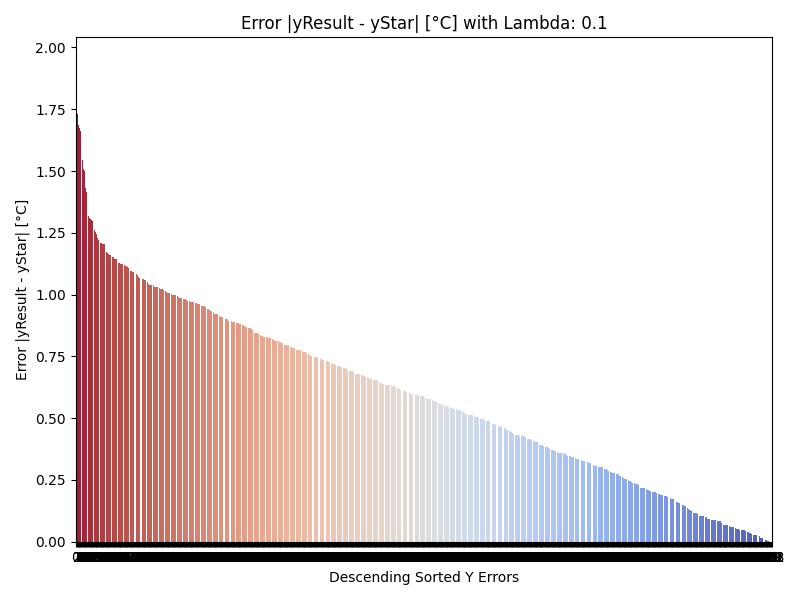
\includegraphics[width=\columnwidth]{pics/ErrorDescWithL_0_1.png}
  \caption{Descending error plot with $\lambda$:0.1}
  \label{fig:fibonacciPlot}
\end{figure}
\begin{figure}[htbp] %or use htbp to place it inside the text blocks
  \centering
  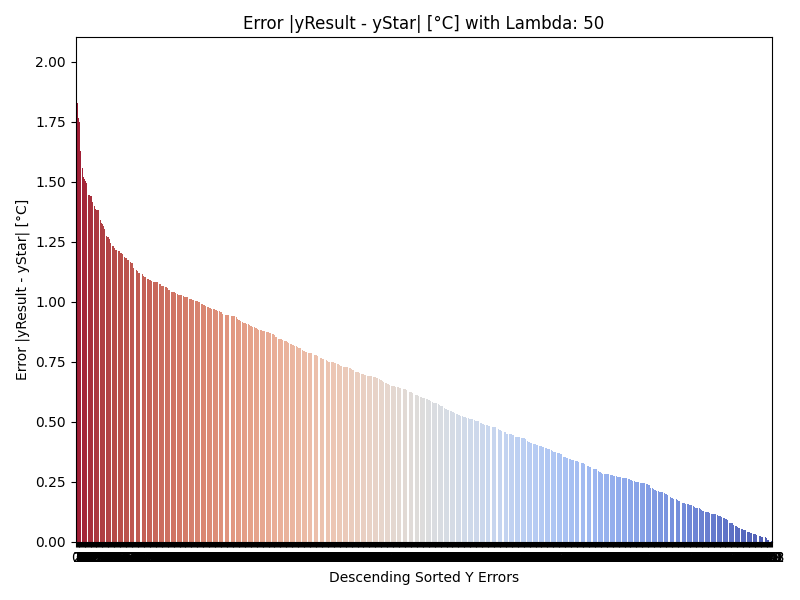
\includegraphics[width=\columnwidth]{pics/ErrorDescWithL_50.png}
  \caption{Descending error plot with $\lambda$:50}
  \label{fig:fibonacciPlot}
\end{figure}
The small changes of the error with a different $\lambda$ is also displayed in Figure 3 and 4. The highest error is exactly on the same position in the heat map, only the value itself changed slightly. 
\begin{figure}[htbp] %or use htbp to place it inside the text blocks
  \centering
  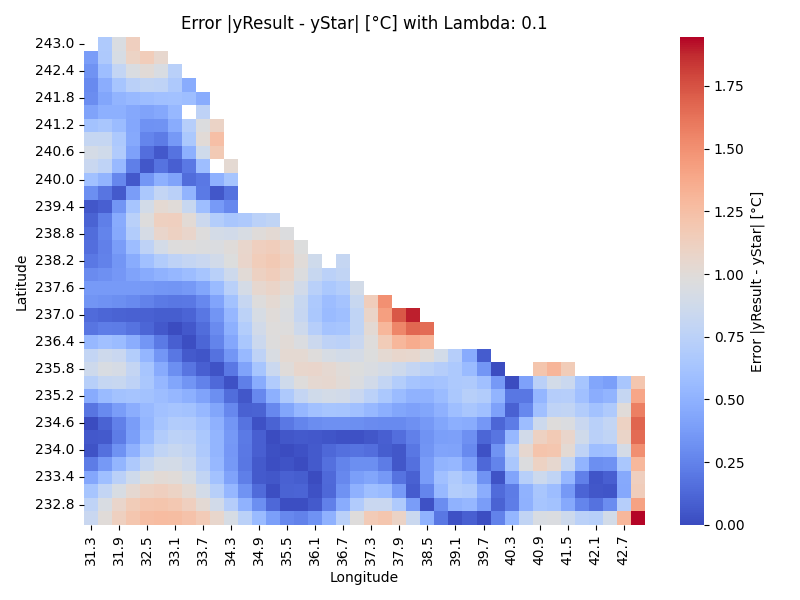
\includegraphics[width=\columnwidth]{pics/ErrorHeatWithL_0_1.png}
  \caption{Heatmap with $\lambda$:0.1}
  \label{fig:fibonacciPlot}
\end{figure}
\begin{figure}[htbp] %or use htbp to place it inside the text blocks
  \centering
  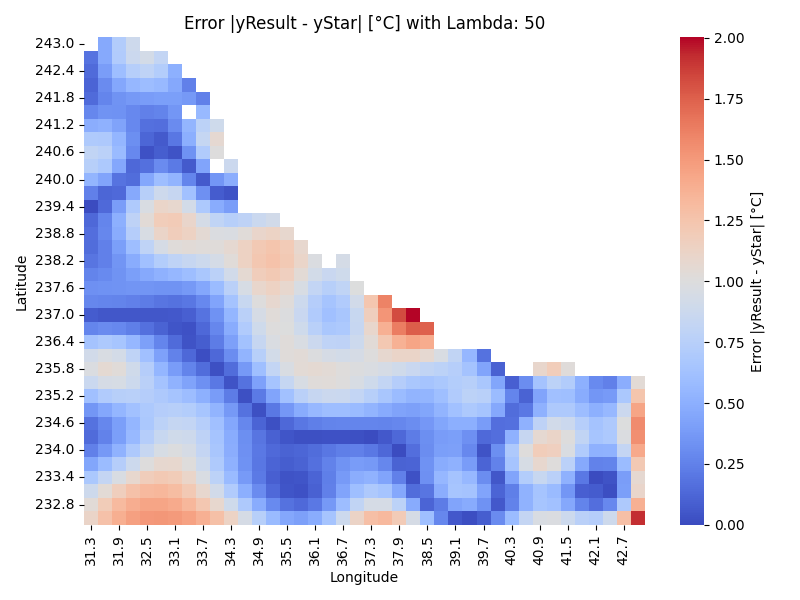
\includegraphics[width=\columnwidth]{pics/ErrorHeatWithL_50.png}
  \caption{Heatmap with $\lambda$:50}
  \label{fig:fibonacciPlot}
\end{figure}
After I made some tests with the different $\lambda$ values I also started to adjust the train step. I reduced the train step to 1 and repeated the tests with different $\lambda$ values. I displayed the results in Figure 5. 
\begin{figure}[htbp] %or use htbp to place it inside the text blocks
  \centering
  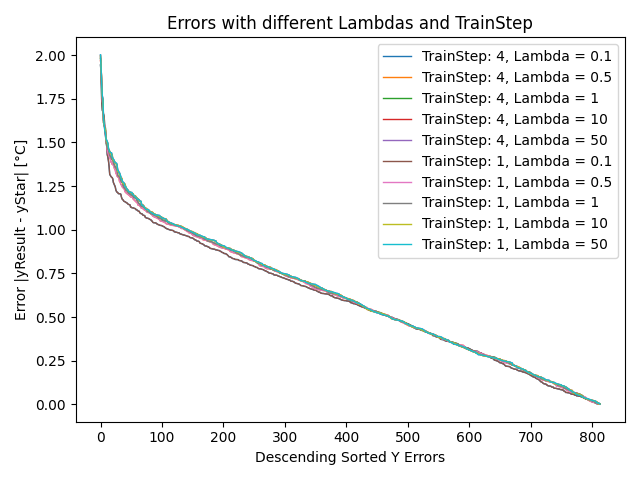
\includegraphics[width=\columnwidth]{pics/LambdaDiff.png}
  \caption{Descending error plot with different lambdas and train steps}
  \label{fig:fibonacciPlot}
\end{figure}
Figure 5 shows, that the changes of the train step and $\lambda$ values only made small adjustment to the results itself. Also the mean values of every tests has only small changes in the value itself. The result of the mean values is displayed in Table 3. 

\begin{table}[htbp]
    \label{tab:alphaBetaParameters}
	\caption{Mean Errors}
	\centering
	\begin{tabular}{llr}
		\cmidrule(r){1-3}
		Train Step & $\lambda$ & Mean\\
		\midrule
		4 & 0.1  & 0.5938 \\
		4 & 0.5  & 0.6117 \\
		4 & 1.0  & 0.6156 \\				
		4 & 10.0 & 0.6195 \\
		4 & 50.0 & 0.6198 \\
		1 & 0.1  & 0.5938 \\
		1 & 0.5  & 0.6117 \\
		1 & 1.0  & 0.6156 \\				
		1 & 10.0 & 0.6195 \\
		1 & 50.0 & 0.6198 \\
		\bottomrule
	\end{tabular}
\end{table}

\subsection{Conclusion}
I had some difficulties with the Implementation of the ridge regression. Especially the augmentation of the values gave me some headache. I even tried to use a \textit{Gaussian Basis Function} with the \textit{Polynomial Basis Function} to create a feature vector. However, all the tries didn't result in a better model. Furthermore, the results were much worse than the straight forward implementation of the feature vector with 1, Latitude and Longitude. One explanation of the error could be the small size of the data set. A larger data set could improve the accuracy of the model. The code of the implementation is in the appendix of this paper. Small side node, I had to remove the correct temperature unit  from the code because it resulted in an \textit{UTF-8} issue. 

%----------------------------------------------------------------------------------------
%	BIBLIOGRAPHY
%----------------------------------------------------------------------------------------

\printbibliography[title={Bibliography}] % Print the bibliography, section title in curly brackets

%----------------------------------------------------------------------------------------


\onecolumn\section*{APPENDIX}
\onecolumn\lstinputlisting{../Task1_BayesTheorem.py}
\onecolumn\lstinputlisting{../Task3_RidgeRegression.py}
\onecolumn\lstinputlisting{../../Modules/RidgeRegression.py}



\end{document}
